\documentclass[11pt,letterpaper]{article}
\usepackage{hyperref}
\usepackage[spanish]{babel}
\usepackage{multirow} 
\usepackage{multicol} 
\usepackage{subfig}
\usepackage{amsmath} % for \text{}
\usepackage{amssymb}
\usepackage{gensymb}
\usepackage{float}
\usepackage{mathrsfs} 
\usepackage{minted}
\usepackage{hyperref}

\usepackage[utf8]{inputenc}
% Control de color en tablas muy versátil.
\usepackage[table]{xcolor}
 % LaTeX


\title{Plantilla Informe}
  
% $Rev: 5 $
% PAQUETES %%%%%%%%%%%%%%%%%%%%%%%%%%%%%%%%%%%%%%%%%%%%%%%%%%%%%%%%%%%%%%%%%%%%
\usepackage{graphicx}
\usepackage{listings}
\usepackage{xcolor}
\usepackage{multicol}
\usepackage{anysize} %Permitir distintas medidas de margenes
\usepackage{framed}
\usepackage{fancyhdr}
\usepackage[spanish]{babel}
\usepackage[utf8]{inputenc}

\fancyhf{} 
\chead{ Proyecto de T\'itulo I \vspace{0.3cm}}
\lhead{
\includegraphics[scale=0.1]{Log.png}}
\rfoot{\thepage}

\renewcommand{\footrulewidth}{0.25pt}

\addtolength{\headheight}{1.4cm}

% CONFIGURACION DE LISTINGS %%%%%%%%%%%%%%%%%%%%%%%%%%%%%%%%%%%%%%%%%%%%%%%%%%%
\newcommand{\AddUserKeywords}[1]{\lstset{morekeywords=[2]{#1}}}
\newcommand{\CodeSize}[1]{\lstset{basicstyle=#1\ttfamily}}
\newcommand{\CommentColor}{\color{green!60!black}}
\newcommand{\StringColor}{\color{red!70!black}}
\newcommand{\UserKeywordsColor}{\color{cyan!50!black}}
\newcommand{\KeywordsColor}{\color{blue}}

\lstdefinelanguage{CSharp}
{
	basicstyle=\small\ttfamily,
	keywordstyle=\KeywordsColor\textbf,
	keywordstyle=[2]\UserKeywordsColor,
	keywordstyle=[3]\StringColor,
	tabsize=2,
	morekeywords={abstract, as, base, bool, break, byte, case, 
		catch, char, checked,class, const, continue, decimal, 
		default, delegate, do, double, else, enum, event, explicit,
		extern, false, finally, fixed, float, for, foreach, get, goto, 
		if, implicit, in, int, interface, internal, is, lock, long,
		namespace, new, null, object, operator, out, override, 
		params, partial, private, protected, public, readonly, ref, return, 
		sbyte, sealed, set, short, sizeof, stackalloc, static, string,
		struct, switch, this, throw, try, typeof, true, uint, ulong, 
		unchecked, unsafe, ushort, using, value, virtual, volatile,
		void, while, where},
	morekeywords=[2]{Main,Console,String},
	morekeywords=[3]{@}, 
	commentstyle=\CommentColor,
	stringstyle=\StringColor,
	sensitive=true,
	morecomment=[l]{//},
	morecomment=[s]{/*}{*/},
	morestring=[b]",
	showstringspaces=false,
	aboveskip=0pt, 
	belowskip=0pt,
	mathescape=true
}

% Set as the default languaje
\lstset{language=CSharp}

\newcommand{\inguandesheader}{
	% Header Facultad Ingenieria Uandes			
	
\includegraphics[scale=0.5]{uandes.pdf}\hspace*{\fill}
}

\newcommand{\evaluationtitle}[2]{
	% T\'itulo
	\begin{center}
	\vspace{1ex}\Large #1\\
	\vspace{1ex}\small #2
	\end{center}
}


\newenvironment{guideexercise}[3]{
	\noindent\textbf{#1}	
	\vspace{-0.3cm}
	\begin{framed}
		\noindent\textsl{Dificultad:} #2\\
		\textsl{Etiquetas:} #3\\	
				
}{
	\end{framed}
	\vspace{0.3cm}
}

\renewcommand{\baselinestretch}{1.5}

\pagestyle{fancy}
\begin{document}

%% COMIENZO PORTADA-----------------------------------------

\begin{titlepage}

\begin{center}

\includegraphics[scale=0.3]{Log.png}\\
% Incrementamos el interlineado:
\vspace{1.0cm} {\LARGE Desatención Racional Para Incentivos ESG\\ Ingenier\'ia Civil Industrial UANDES\\

\vspace{1.5cm} \LARGE{Por:\\ Ezequiel Ortiz Torres \\ Gu\'ia: \\ Sebasti\'an Cea}

\vspace{2.3cm}

\vspace{.5cm} \today

\end{center}
\end{titlepage}

 %%%% FIN PORTADA ------------------------------------------

\tableofcontents
\newpage


\section{Introducción}

\subsection{Desatención racional}

La desatención o inatención racional ha sido ampliamente estudiada, para poder explicar ciertos fenómenos de la economía y el actuar de los individuos. Por ejemplo, los compradores pueden comprar productos innecesariamente caros debido a que no notan si el impuesto sobre las ventas está incluido o no en los precios establecidos (Chetty, Looney y Kroft 2009). Otro caso son los compradores de autos usados, que centran su atención en el dígito más a la izquierda del odómetro (Lacetera, Pope y Sydnor 2012) o los compradores que utilizan páginas de e-commerce limitan su atención a un número relativamente pequeño de sitios web (De Los Santos, Hortaçsu y Wildenbeest 2012).

En sencillo, el estudio de la desatención racional busca explicar las decisiones ``erradas" de las personas cuando enfrentan algún problema sin querer decir que son personas irracionales. 

Este estudio, quiere exponer de que forma las decisiones de los inversionistas se ven condicionadas por dos tipos de incentivos: económicos y sustentables.

Para poder obtener datos y analizar la desatención racional, se creó un juego compuestos por tareas que deberá resolver el inversionista. Originalmente, el juego propuesto por Dewan y Neligh contaba con dos tipos de tareas, contar puntos y ángulos,  y un solo incentivo, el económico. 

El juego propuesto en esta memoria consta de un solo tipo de tarea, contar puntos, y dos incentivos, mateniendo el económico y agregando el sustentable.

La motivación principal es determinar si el segundo criterio suma o resta para la atención que los inversionistas prestaban en el juego y como se desempeñaban. Utilizando la ecuación de costos cuadrática y su ecuación de estimación se estimaron los parámetros, obteniendo los costos estimados, logrando argumentos para desembolver el análisis.

Por motivos de disponibilidad y accesibilidad a la información, se llevaron a cabo dos simulaciones utilizando la base de datos original, aplicando el segundo incentivo, y desarrollando la forma en que este afectaba a la regresión.

Antes de comenzar con las explicaciones específicas del experiemento, debemos entender que son los críterios ESG y todo lo que los envuelve.

\subsection{El Ecosistema ESG}

Se llamará Ecosistema ESG a todo lo que envuelve la toma de decisiones con respecto a los proyectos sustentables. Los actores tienen distintos niveles de importancia en esta área, y cumplen roles que son detallados a continuación. 

En primer lugar, los criterios ESG tienen origen en los años 60, posterior a la guerra de vietnam, cuando los universitarios estadounidenses se vieron envueltos en protestas exigiendoles a las universidades no invertir en instrumentos militares según señala la página del Banco Santander (2020), en su artículo sobre la definición de estos criterios. 

Además, los 3 factores en que se fundamentan estos criterios son los siguientes:

\begin{enumerate}

\item El factor ambiental (E), para tomar decisiones en función de cómo afectan las actividades de las empresas en el medio ambiente.
\item El factor social (S), para tener en cuenta la repercusión que tienen en la comunidad las actividades desempeñadas por la compañía, por ejemplo, en términos de diversidad, derechos humanos o cuidados sanitarios.
\item El factor de gobierno (G), que estudia el impacto que tienen los propios accionistas y la administración, y se basa en cuestiones como la estructura de los consejos de administración, los derechos de los accionistas o la transparencia, entre otros.

\end{enumerate}

\subsubsection{Descripción del Ecosistema:}

\subsubsection{Fondos de Inversión:}

Son los tomadores de decisiones por definición. Como entidad, funcionan a través de mediciones llevadas a cabo por instrumentos de análisis tanto humanos como a nivel de software. Esto determina un orden jerárquico entre las primeras evaluaciones hasta la decisión final de inversión.

\subsubsection{Gobierno:}

El gobierno toma parte importante en el ecosistema ESG. El poder legislativo a través de leyes y regulaciones, dicta argumentos para que las empresas guíen sus actividades en pos de características sustentables. Un ejemplo de esto son la ley de fomento al reciclaje, contenida en la ley N° 20.920 (Biblioteca del Congreso Nacional, 2016) o en el plan de Acción Nacional de Cambio Climático (PANCC 2017-2022), que contribuye a uno de los más reelevantes objetivos del desarrollo sustentable: aportar a la reducción del calentamiento global. 

Otro arista que destaca es la CORFO (Corporación de fomento a la producción) que constantemente está llamando a participar por fondos, como capital semilla entre otros, con el requisito de tener características sustentables dentro de los proyectos. 

\subsubsection{Proyectos y empresas:}
En este nivel se encuentran todos los emprendedores, las pymes y también los negocios medianos y grandes (a través de la venta de bonos verdes por ejemplo), quienes presentan una oportunidad a los fondos, desencadenando todo lo anterior. Sin las ideas sustentables no existe análisis ni ecosistema. 

Un caso de empresa que profesa con este objetivo es Wild Lama, la cuál basa sus productos en 5 pilares sustentables: material reciclado, fibras sustentables, comercio justo, material orgánico o productos con causa. De hecho, el 97,89\% de sus productos fueron fabricados con alguno de estos pilares (pagina oficial de wild lama). Actualmente se encuentran levantando cápital por USD 3 millones, con asistencia del holding Fynsa.


Para describir mejor lo anterior, se presenta un esquema de elaboración propia con el objetivo de explicar a priori, lo que se espera encontrar en este ecosistema, y postula la hipótesis de que todo instrumento de medición será observado con ojos muy distintos dependiendo del nivel y el rol desempeñado, y buscará establecer recomendaciones para los distintos actores involucrados.

\begin{itemize}
    \item Esquema Ecosistema ESG
        \begin{figure}[h]
            \centering
            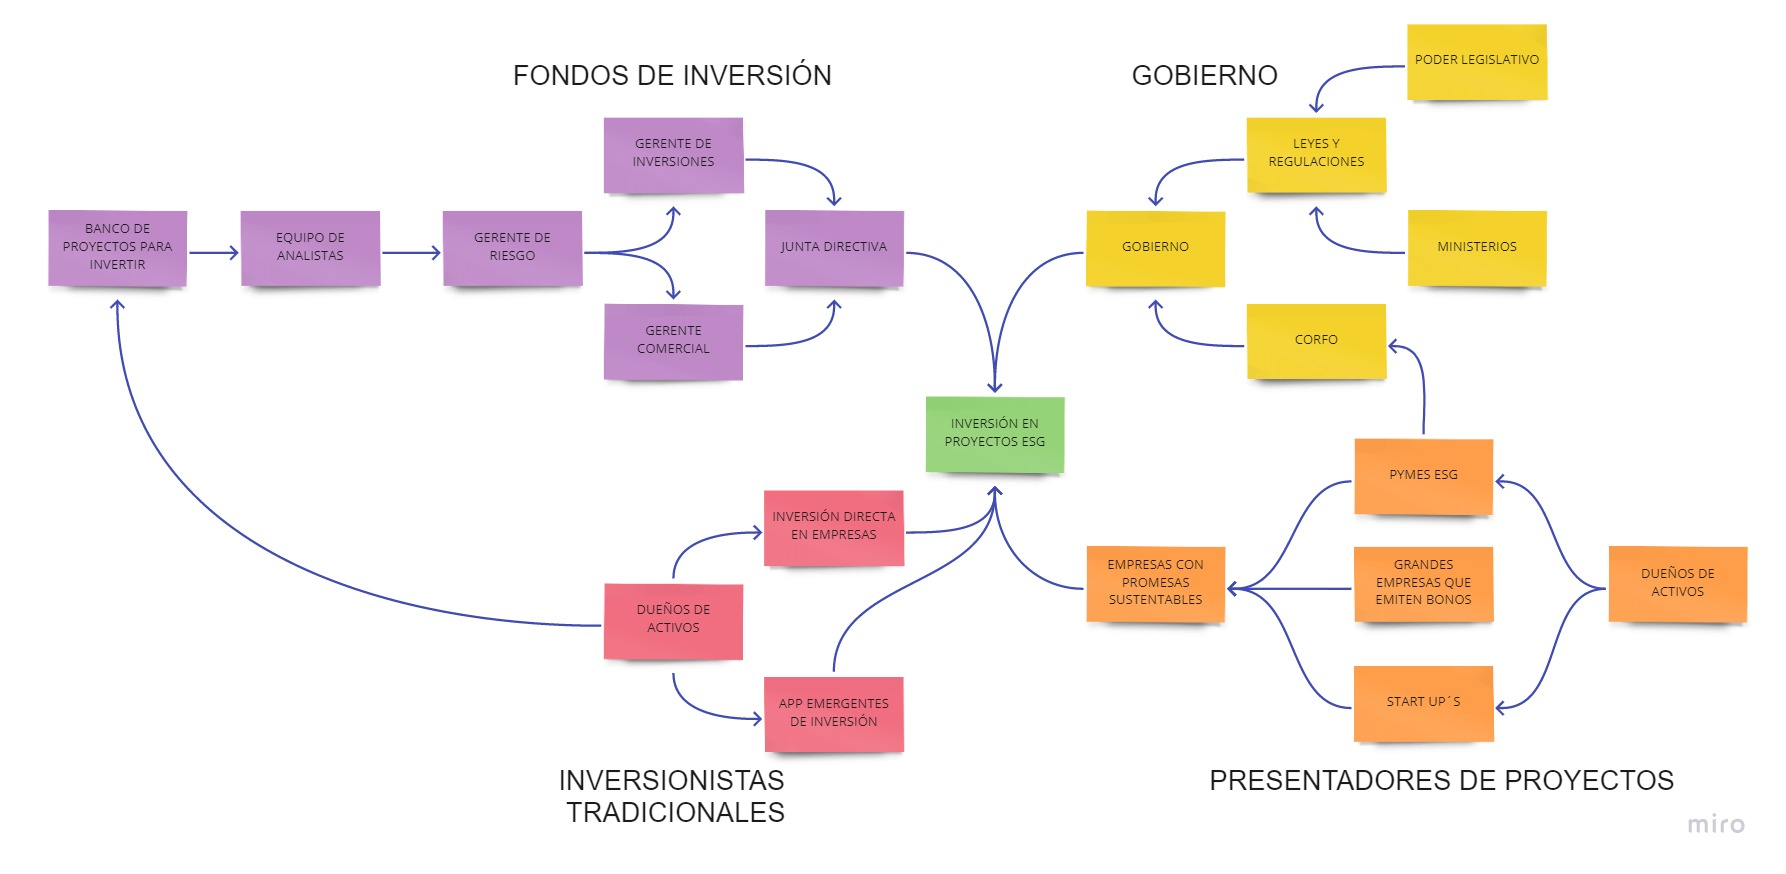
\includegraphics[scale=0.2]{Concept Map - Frame 1.jpg}
            \caption{Ecosistema ESG}
        \end{figure}
\end{itemize}

En este esquema, los actores pueden ser los inversionistas o dueños de activos que trabajan su capital de distintas formas. En rojo aparecen los inversionistas más modernos y bajo el modelo de "cualquiera puede invertir", que depositan su dinero en aplicaciones modernas como Fintual o Racional. También, los inversionistas más grandes o convencionales que invierten a través de fondos de inversión, señalados en color morado, las cuales realizan contribuciones y compras de bonos en proyectos ESG.

En amarillo está el gobierno, que además de regular a través de la legislación del país, también invierte con criterios ESG, y tiene instrumentos como CORFO que aporta al desarrollo de la pymes. 

Finalmente, en Naranjo aparecen las empresas como tal, que tienen las ideas sustentables y que se desempeñan gracias a las inversiones como el ejemplo de Wild Lama.



\section{Marco Teórico.}

El marco teórico está basado en el artículo de Ambuj Dewan y Nathaniel Neligh, \textit{Estimating information cost functions in models of rational inattention} ya que es el mismo experimento (y es el documento base de esta memoria), con el valor agregado de incorporar una variable de medición de sustentabilidad en la experienca. Con esto, se otorga mayor contexto a la experiencia en general.

\subsection{Tareas de conjetura uniforme}

La tarea escogida para evaluar a los tomadores de decisión (TD) responde a un marco general de desatención racional discreta. En partícular, buscamos explicar este fenómeno a través de la ya más común teoría de la inatención racional (Sims, 2003, 2006; Caplin y Dean, 2015; Matejka y McKay, 2015), la cuál postula que las personas eligen racionalmente la infomación a la que asisten, intercambiando los costos de prestar más atención con los consiguientes beneficios de mejores decisiones (Dean y Neligh, 2019).

Ahora, considere una tarea $\theta$ $\in$ $\bullet$ donde existe un estado real desconocido del mundo (más adelante, este mundo es la prueba que realiza el (TD)) y el (TD) tiene que identificar cual es este estado. La probabilidad de ocurrencia del estado $n$ está representado por: 
$${Pr}(\theta) = \frac{1}{n}, \forall\theta\in\bullet.$$


En otras palabras, existen $n$ estados posibles, los cuales son a priori equiprobables, por lo tanto, la información previa del (TD) sobre el estado del mundo es uniforme. Si bien es cierto, con el correr de la repeticiones de la experiencia el (TD) puede adquirir nueva información (por ejemplo, la vista se puede acostumbrar a la cantidad de puntos), es irrelevante considerarla ya que también tiene el caracter de ser uniforme.

El (TD) recibe una recompensa $r$ por identificar correctamente el estado y nada por equivocarse. El objetivo del TD será maximizar la probabilidad de identificar este estado correcto, a lo que denominaremos como performance, estimando los costos en los que incurre para recopilar la información necesaria para encontrar el estado verdadero. las tareas con esta configuración son Las que llamaremos tareas de conjetura uniforme.

La performance del individuo, será determinada por la elección con la que este estructura la información, donde se enumera la probabilidad de encontrar el estado correcto, dada la conjetura del TD denotada como $a$ $\in$ $\bullet$

Formalmente, una estructura de información es una colección de probabilidades condicionales $(q_i,_j)$, donde $i,j=1,...,n$ donde $q_i,_j$ $=$ Pr($a$=$\theta_i$ $|$ $\theta$=$\theta_j$). Cuando el TD debe adivinar o responder, la creencia sobre las probabilidades de cada uno de los estados posibles, está dada por Pr($\theta$=$\theta_i$ $|$ $a$=$\theta_j$). Aplicando el teorema de Bayes, se puede demostrar que esto es igual a $\cfrac{q_i,_j}{\sum_{k=1}^{n}q_k,_j}$ refiriendose a esta distribución de probabilidad del estado del mundo condicionado por la suposición del TD como su creencia posterior.

Con esto, podemos estimar cuales serán los costos de la información a través de la performance del TD.

La supocisión del TD será correcta cuando $a=\theta$, de lo contrario será incorrecta. Por lo tanto, la performance P estará dada por:
\begin{center}
    $P=\cfrac{1}{n}\sum_{i=1}^{n}q_i,_j$
\end{center}
Luego, el objetivo del TD será elegir P maximizando:
\begin{center}
$rP-C(P)$
\end{center}
donde $r>0$ es la recompensa, $P \in [0,1]$ es la performance elegida por el TD y la funcion $C (\cdot)$ es un costo asociado. Se denota por $P(r)$ la elección de $P$ por parte del TD para una $r$ dada, y se llamará al mapeo resultante de recompensa, como la performance de la función de performance.
Un ejemplo de una tarea de conjetura uniforme, es la empleada en el experimento base. La tarea se trata de contar "puntos", el TD se enfrenta a una pantalla que muestra una disposición aleatorea de puntos. El objetico será determinar en número de puntos que muestra la pantalla, cuya cantidad está entre 38 y 42, inclusive, y la cantidad es igualmente posible para cualquiera de los números. Se recibirá una recompensa por cada vez que acierte a la cantidad de puntos, y no recibe nada en caso de errar. Los costos para esta tarea podrían ser el esfuerzo por contar, los costos cognitivos de emplear una heurística para estimar o adivinar, o el tiempo dedicado a tratar de determinar el número de puntos.

\subsection{Prueba de inatención racional}

Se debe testear la existencia de la función de costos que sigue el TD, para determinar su existencia. Caplin y Dean (2015) demuestran en su primer teorema, que el comportamiento observado es consistente con un marco de inatención racional de costos separables aditivamente si y solo si satisface las condiciones NIAC \textit{"no improving attention cycles"} y NIAS \textit{"no improving action switches"}. 

La hipotesis más reelevante del experimento dice que la asignación eficiente de la atención consiste en prestar más atención o esforzarse más por realizar bien la experiencia cuando es más valioso hacerlo, es decir, cuando las recompensas son mayores. Para formalizar esto, tomaremos la siguiente proposición.


\vspace{0.5cm}

\textbf{Proposición 1.} El comportamiento del TD es consistente con NIAC si $P(r)$ no es decreciente en $r$.

\vspace{0,5cm}

NIAC descarta las respuestas negativas al aumento de los incentivos, por ejemplo, al estar estresado por las apuestas más altas. En otras palabras, el TD siempre deberá tener mayor performance a mayor incentivo.

Optener conjeturas de manera optima, significa que una conjetura correcta es más probable que obtner una incorrecta, es decir, cambiar una conjetura no conllevará a un mejor resultado. Para formalizar.

\vspace{0,5cm}

\textbf{Proposición 2.} El comportamiento del TD es consistente con NIAS si $\forall r, \forall x \in \bullet$,


y $\forall y \in \bullet, Pr(\theta=x| a=x)\geq Pr(\theta=y | a=x)$

\vspace{0,5cm}

Dicho de otra manera, se satisface NIAS si y solo si los resultados basados en la experiencias del TD se maximizan con respecto al estado de adivinación. Con esto, se descarta el uso sistemático de la información, como sería cambiar mentalmente dos estados del mundo. 

Por lo tanto, un TD será racionalmente desatento si satisface las proposiciones 1 y 2, es decir, un tomador de decisión responde a incentivos, y siempre estará más seguro de responder de forma empírica que adivinando.

\subsection{Capacidad de respuesta}

Si un TD selecciona un mismo nivel de desempeño independiente de la recompensa, se dice que es consistente con la falta de atención racional. Por ejemplo, si el individuo no observa el nivel de incentivo, no discriminará en el nivel de esfuerzo para realizar la experiencia. El caso interesante, es cuando el TD modifica su comportamiento según la recompensa.
Por lo tanto, si $r_2$ $>$ $r_1$, entonces, $P(r_2)$ $>$ $P(r_1)$.

\subsection{Continuidad y Convexidad}

En el marco de inatención racional, la continuidad de una función de costos implica que un aumento pequeño de información adicional, aumenta el costo total de la información en una cantidad pequeña. En tanto, la convexidad implica que el costo marginal de la información estña aumentando, es decir, mientras más información se adquiere, más díficil (costoso) se vuelve adquirir nueva información. Esto se puede comprobar según el comportamiento de un TD. Se denota $P * (r)$ la maximización de la performance del TD para cada $r$, entonces, la función de costos $C(\cdot)$ se comporta bien si es continua y convexa en $[0,1]$, es estrictamente creciente y estrictamente convexo en $(\cfrac{1}{n},1$) y tiene un mínimo global en $\cfrac{1}{n}$. Formalizando,

\vspace{0,5cm}

\textbf{Proposición 3.} Si $C(\cdot)$ se comporta bien, entonces $P*(r)$ es continuo.

\vspace{0,5cm}

Como el TD siempre buscará maximizar la utilidad, se rechazará el buen comportamiento de la función de costo si se observa que la función de desempeño $P(r)$ es discontinua.

\subsection{Inclusión de un nuevo incentivo}

Si bien es cierto, un nuevo incentivo implica que $r$ se comportará como una función $F(r)$, $r = r_1 + r_2$ por ejemplo, siendo $r_2$ un incentivo externo de caracter colateral, como un pilar sustentable, especificar un tipo de retorno, o entregar una nueva característica del proyecto, las funciones no van a cambiar en su escencia y el comportamiento se va a regir de la misma forma, pero la válidación de la recompensa será una combinación de estos dos incentivos. 

Será interesante evaluar la forma en que conectarán estas señales para el TD para concluir de que forma afectará una característica alterna. Adicionalmente, el TD tendrá preferencia por alguno de las dos características, y esta información si la podemos conocer a priori. Formalizando, si la función de costo es cuadrática toma la forma dependiente en la \emph{performance} o desempeño $P$ de la siguiente manera:

$$C(P)=\begin{cases}c\cdot(P-d)^2& P\geq d\\ 0&\text{otro caso}\end{cases}$$

Usando la Proposición 4 de Dewan y Neligh tenemos que la $P$ óptima en función del incentivo es:

$$P^*(r)=\begin{cases}\frac{r}{2c}+d& r\leq 2c(2-d)\\ 1&\text{otro caso}\end{cases}$$

Si tenemos canales de incentivo, ¿Será que la nueva función de desempeño es?

$$P^*f(r_1,r_2)=\begin{cases}\frac{f(r_1,r_2)}{2c}+d& r\leq 2c(2-d)\\ 1&\text{otro caso}\end{cases}$$

y que forma funcional tiene $f$. Por ejemplo, aditiva, es decir $f(r_1,r_2)=r_1+r_2$. ¿Cómo queda la función de costo de origen?


\section{Función de Costos Cuadrática.}

La función de costos cuadrática se utilizará como objeto de análisis en cuanto al desempeño o performance del TD muestre. 

La función de costos cuadrática está dentro del amplio espacio admisible, dado que cumple con $\longrightarrow \mathbb R$ función de costo $C:[0,1]$, lo cuál conduce a un comportamiento consistente con NIAS y NIAC. (Dewan y Neligh, 2019)

Además, si C es diferenciable, entonces el problema del TD puede resolverse utilizando el cálculo. Esta característica da como resultado poder encontrar la función C a través del desempeño observado. (función Inversa)

\vspace{0,5cm}

\textbf{Proposición 4.} Suponga que C se comporta bien (continua y creciente) y es diferenciable.

\begin{center}
    $P*(r) = (C')^{-1}$ 
\end{center}

Entonces, para todo r tal que

\begin{center}
    $C'(\cfrac{1}{n})<r<\lim_{x\uparrow1} C'(x)$
\end{center}

Además,

\begin{center}

$P*(r) = 1$  para  $r$  $\geq \lim_{x \uparrow  1} C'(x)$

\end{center}

\vspace{0,5cm}

Tomando la condición de primer orden en la maximización de la función y el hecho de que la performance no puede ser mayor a 1, podemos establecer que el costo se puede deducir invirtiendo e integrando la función de desempeño o performance observada, siempre y cuando dicha función sea estrictamente creciente y continua en los incentivos.

\subsection{Nuevo incentivo en la función de costos}

Ya habiendo establecido que la función que vamos a utilizar es la función de costos cuadrática, queda observar como queda utilizando el incentivo r como una función.

Para esto podemos separar en dos funciones de retorno el análisis. En primera instancia el retorno que mide la sustentabilidad sumará\footnote{El TD cree que el retorno de sustentabilidad aporta al retorno económico} al retorno original al cuál estuvieron sometidos los inversionistas. Formalizando,

\vspace{0,5 cm}

\textbf{Proposición 5.} Si $f(r)$ es aditiva, entonces $r = r_1 + r_2$

\vspace{0,5 cm}

El caso opuesto, la hipotesis es que el retorno sustentable va a restar\footnote{No es una resta enrealidad, supone que un retorno económico se puede ver afectado negativamente por un retorno sustentable} al retorno original. Formalizando,

\vspace{0,5 cm}

\textbf{Proposición 5.} Si $f(r)$ es diminutiva, entonces $r = r_1 - r_2$

\vspace{0,5 cm}

\subsection{El problema de maximización}

Si el tomador de desición es concencuente con todo lo que se describió anteriormente, entonces enfrentará el siguiente problema de maximización.

\begin{center}

    max z: \hspace{0,5cm}   $r*P - C(P)$, con $P \in$ $[0,1]$
    
\end{center}

Además, si la función de costos C(P) es igual a:

\begin{center}

    $C(P) = c*(P - d)^2$
\end{center}

Siendo,

\begin{itemize}
    \item r: nivel de incentivo.
    \item P: Probabilidad que mide la performance según las respuestas del TD.
    \item d: es la cantidad de información que está disponible.
    \item c: el costo marginal que regula la obtención de nueva información.
\end{itemize}
    
Luego, reemplazando

\begin{center}
    $r*P - c*(P - d)^2$
\end{center}

Utilizando la condición de primer orden (C.P.O):

\begin{center}
    $\cfrac{\partial z}{\partial P}$ = $0$
    
\vspace{0,5cm}
    
    $\Rightarrow$ $r - 2c(P-d) = 0$
    
\end{center}

Despejando la performance,

\begin{center}
    $P'(r) = \cfrac{r}{2c} + d$
\end{center}

Dado que la performance es un dato conocido para nosotros, obtenido de las respuestas al experimento, los valores de c se pueden estimar aplicando regresiones como veremos más adelante.

Ahora, aplicaremos las dos funciones de retorno de la hipotesis a la primera derivada quedando,

\vspace{0,5 cm}
\textbf{Proposición 6.} Si $f(r) = r_1 + r_2$, entonces la  C.P.O queda $P'(f(r)) = \cfrac{r_1 + r_2}{2c} + d$
\vspace{0,5 cm}


Si integramos la C.P.O 

\begin{equation}
    \int_{}{} P'(f(r)) \cdot dr
\end{equation}

Entonces, el problema de maximización z' queda

\begin{equation}
    max \hspace{0,3cm}z' \hspace{0,5cm} (r_1 + r_2)\cdot P - C(P)
\end{equation}

De la misma forma,

\vspace{0,5 cm}
\textbf{Proposición 7.} Si $f(r) = r_1 - r_2$, entonces la  C.P.O queda $P'(f(r)) = \cfrac{r_1 - r_2}{2c} + d$
\vspace{0,5 cm}


Si integramos la C.P.O 

\begin{equation}
    \int_{}{} P'(f(r)) \cdot dr
\end{equation}

Entonces, el problema de maximización z' queda

\begin{equation}
    max \hspace{0,3cm}z' \hspace{0,5cm} (r_1 - r_2)\cdot P - C(P)
\end{equation}

Lo interesante es calcular las derivadas de segundo orden (C.S.O) con respecto a $r_1$ y a $r_2$, ya que en el primer caso, es decir, cuando estas se suman, los resultados son iguales.


\vspace{0,5 cm}
\textbf{Proposición 8.} Si $f(r) = r_1 + r_2$, entonces la  C.S.O quedan:

\begin{equation} 
    \cfrac{\partial P'(f(r))}{\partial r_1} = \cfrac{1}{2c}, \hspace{0,3 cm} manteniendo \hspace{0,2 cm} r_2 \hspace{0,2 cm}constante
\end{equation}

\begin{equation} 
    \cfrac{\partial P'(f(r))}{\partial r_2} = \cfrac{1}{2c}, \hspace{0,3 cm} manteniendo \hspace{0,2 cm} r_1 \hspace{0,2 cm}constante
\end{equation}

\vspace{0,5cm}

Pero cuando aplicamos la C.S.O en el segundo caso, los resultados son distintos.

\vspace{0,5 cm}
\textbf{Proposición 8.} Si $f(r) = r_1 - r_2$, entonces la  C.S.O quedan:

\begin{equation} 
    \cfrac{\partial P'(f(r))}{\partial r_1} = \cfrac{1}{2c}, \hspace{0,3 cm} manteniendo \hspace{0,2 cm} r_2 \hspace{0,2 cm}constante
\end{equation}

\begin{equation} 
    \cfrac{\partial P'(f(r))}{\partial r_2} = -\cfrac{1}{2c}, \hspace{0,3 cm} manteniendo \hspace{0,2 cm} r_1 \hspace{0,2 cm}constante
\end{equation}

Esto, lo podemos utilizar de test para predecir que factores de sustentabilidad restan retorno económico, y con esto, establecer ciertos parámetros de medición.

\section{Ecuación de Estimación Econométrica}

Luego, siguiendo el paper de estimación de costos de Dewan y Neligh, para la función de costos cuadrática se utiliza la siguiente ecuación de estimación basado en la performance o desempeño:

\begin{equation}
    P_t = \beta_0 + \beta_1 r_t
\end{equation}

Con esto, la función de estimación de costos queda:

\begin{equation}
    \Hat{C}(P) = \cfrac{1}{2\Hat{\beta_1}}(P^2 - 0.04) - \cfrac{\Hat{\beta_0}}{\Hat{\beta_1}}(P-0.02)
\end{equation}

Para la estimación de los betas, se utilizará el programa Stata, ya que conocemos los incentivos y la \textit{performance} o desempeño de cada uno de los individuos.



\section{Diseño Experimental: Conteo de puntos}

El experimento que se implementa en esta memoria, está basado por completo en el que realizaron Dewan y Neligh (2019). 

\subsection{Experimento Original}

El experimento original invólucra dos tipos de tareas de percepción, cada una de las cuales tenía una recompensa potencial. En el primer tipo de tarea, a los sujetos se les mostró una pantalla con una distribución aleatorea de puntos y se les pidió que determinaran la cantiad de puntos en la pantalla, ya sea de forma empírica o adivinando. Este número de puntos estaba entre 38 y 42 inclusive en todas las repeticiones, y cada número era equiprobable de ser la respuesta correcta. Los individuos estaban en conocimiento de todos estos antescendentes, sin engaños ni información oculta.

Una segunda tarea involucraba identificar ángulos, la cuál no tiene reelevancia para esta parte de la investigación.

Antes de comenzar cada tarea n, con n $\in$ $[1,100]$, se mostraba una recompensa que denominaremos r, con r $\in$ $[1,100]$, referente al nivel de incentivo, de forma resaltiva y grande, (como muestra la Fig.2) durante 3 segundos, para luego dar paso a una segunda pantala que muestra la distribución de puntos aleatoreos (como muestra la Fig.3). Ambas imagenes son del texto \textit{Estimating information cost functions in models of rational inattention (Dewan y Neligh, 2019)}. Esto fué así con el objetivo de que el individuo observara plenamente el incentivo, y lo tuviese claro antes de comenzar con la tarea. Este nivel de incentivo nunca dejaba de estar presente en la pantalla, aun cuando cambiaba a la segunda pantalla, asegurando que el sujeto no necesitaran memorizar el incentivo.


    \begin{figure}[h]
        \centering
        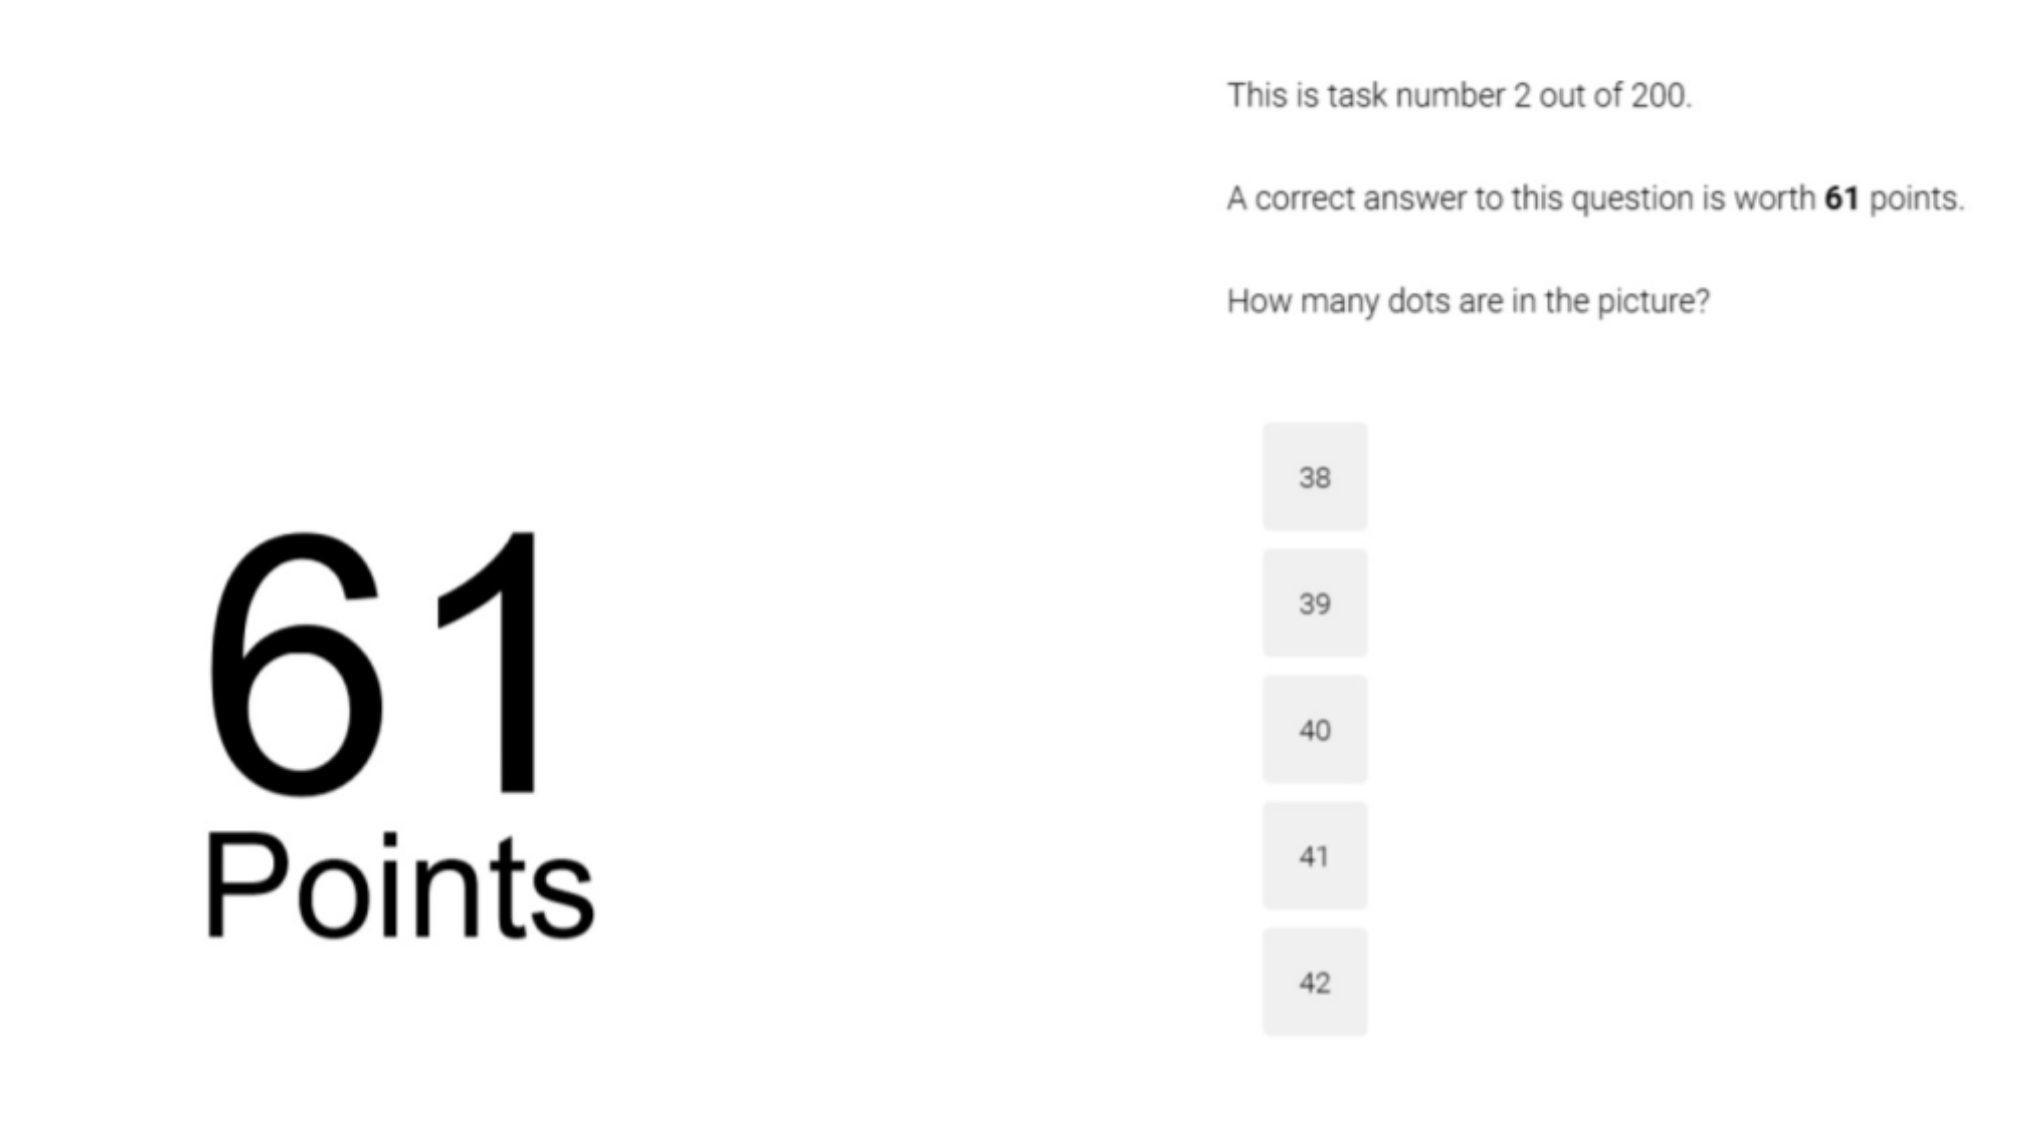
\includegraphics[scale=0.5]{IMAGEN NIVEL DE INCENTIVO.png}
        \caption{Pantalla 1, Nivel de incentivo}
    \end{figure}


Este nivel de incentivo, se puede ver también como la probabilidad de ganar el juego $Pr(Y_t=1|r_t)$, donde $P_r$ es la probabilidad de acertar $Y_t$ dado el incentivo $r_t$. (referenciar la parte en que esto se explica en el marco teorico)
El tiempo no era una limitante para responder, dado que los individuos tenían todo el tiempo que necesitaran para determinar la cantidad de puntos, y así pasar a la pantalla siguiente. Accedían a la recompensa potencial al responder correctamente, de lo contrario, no obtenían recompensa por esa tarea. No se les informaba si respondieron bien o mal hasta el termino de todos los conteos.
Los individuos fueron sometidos a las 100 tarea del conteo de puntos de forma seguida, y el nivel de incentivo aparecía de forma aleatorea, que como ya dijimos, podía ser entre 1 y 100 inclusive.
Los bloques de tareas se equilibraron por nivel de incentivo para garantizar aproximadamente el mismo nivel de variación en los incentivos a lo largo del experimento. A los sujetos se les mostró primero cada uno de los 50 niveles de incentivos impares entre 1 y 100 en un orden aleatorio, y luego se les mostró cada uno de los 50 niveles de incentivos pares entre 1 y 100 en un orden aleatorio. Esto se repitió (en un orden aleatorio diferente) para las siguientes 100 tareas.
Las ganancias experimentales se determinaron de la siguiente manera. Una tarea de la primera mitad del experimento y una tarea de la segunda mitad del experimento se seleccionaron al azar para el pago. El nivel de incentivo de cada tarea seleccionada determinaba la probabilidad de ganar uno de los dos premios monetarios. Por ejemplo, si la primera tarea seleccionada tenía un nivel de incentivo de 84 y se respondió correctamente, y la segunda tarea seleccionada tenía un nivel de incentivo de 33 y se respondió incorrectamente, esto le daría al sujeto un 84\% de probabilidad de ganar el primer premio. y un 0\% de probabilidad de ganar el segundo premio. La determinación de las ganancias de esta manera aseguró que las ganancias esperadas fueran lineales en el nivel de incentivos, lo que obvió la necesidad de obtener preferencias de riesgo. En otras palabras, esto aseguró que bajo el supuesto de la teoría de la utilidad esperada, conociéramos las utilidades de los sujetos (excluyendo los costos de información) (hasta una constante multiplicativa). Así, la relación estimada entre desempeño y nivel de incentivo para cada sujeto podría considerarse una estimación válida de su función de desempeño, sin necesidad de aplicar ninguna transformación adicional (Dewan y Neligh, 2019).



    \begin{figure}[h]
        \centering
        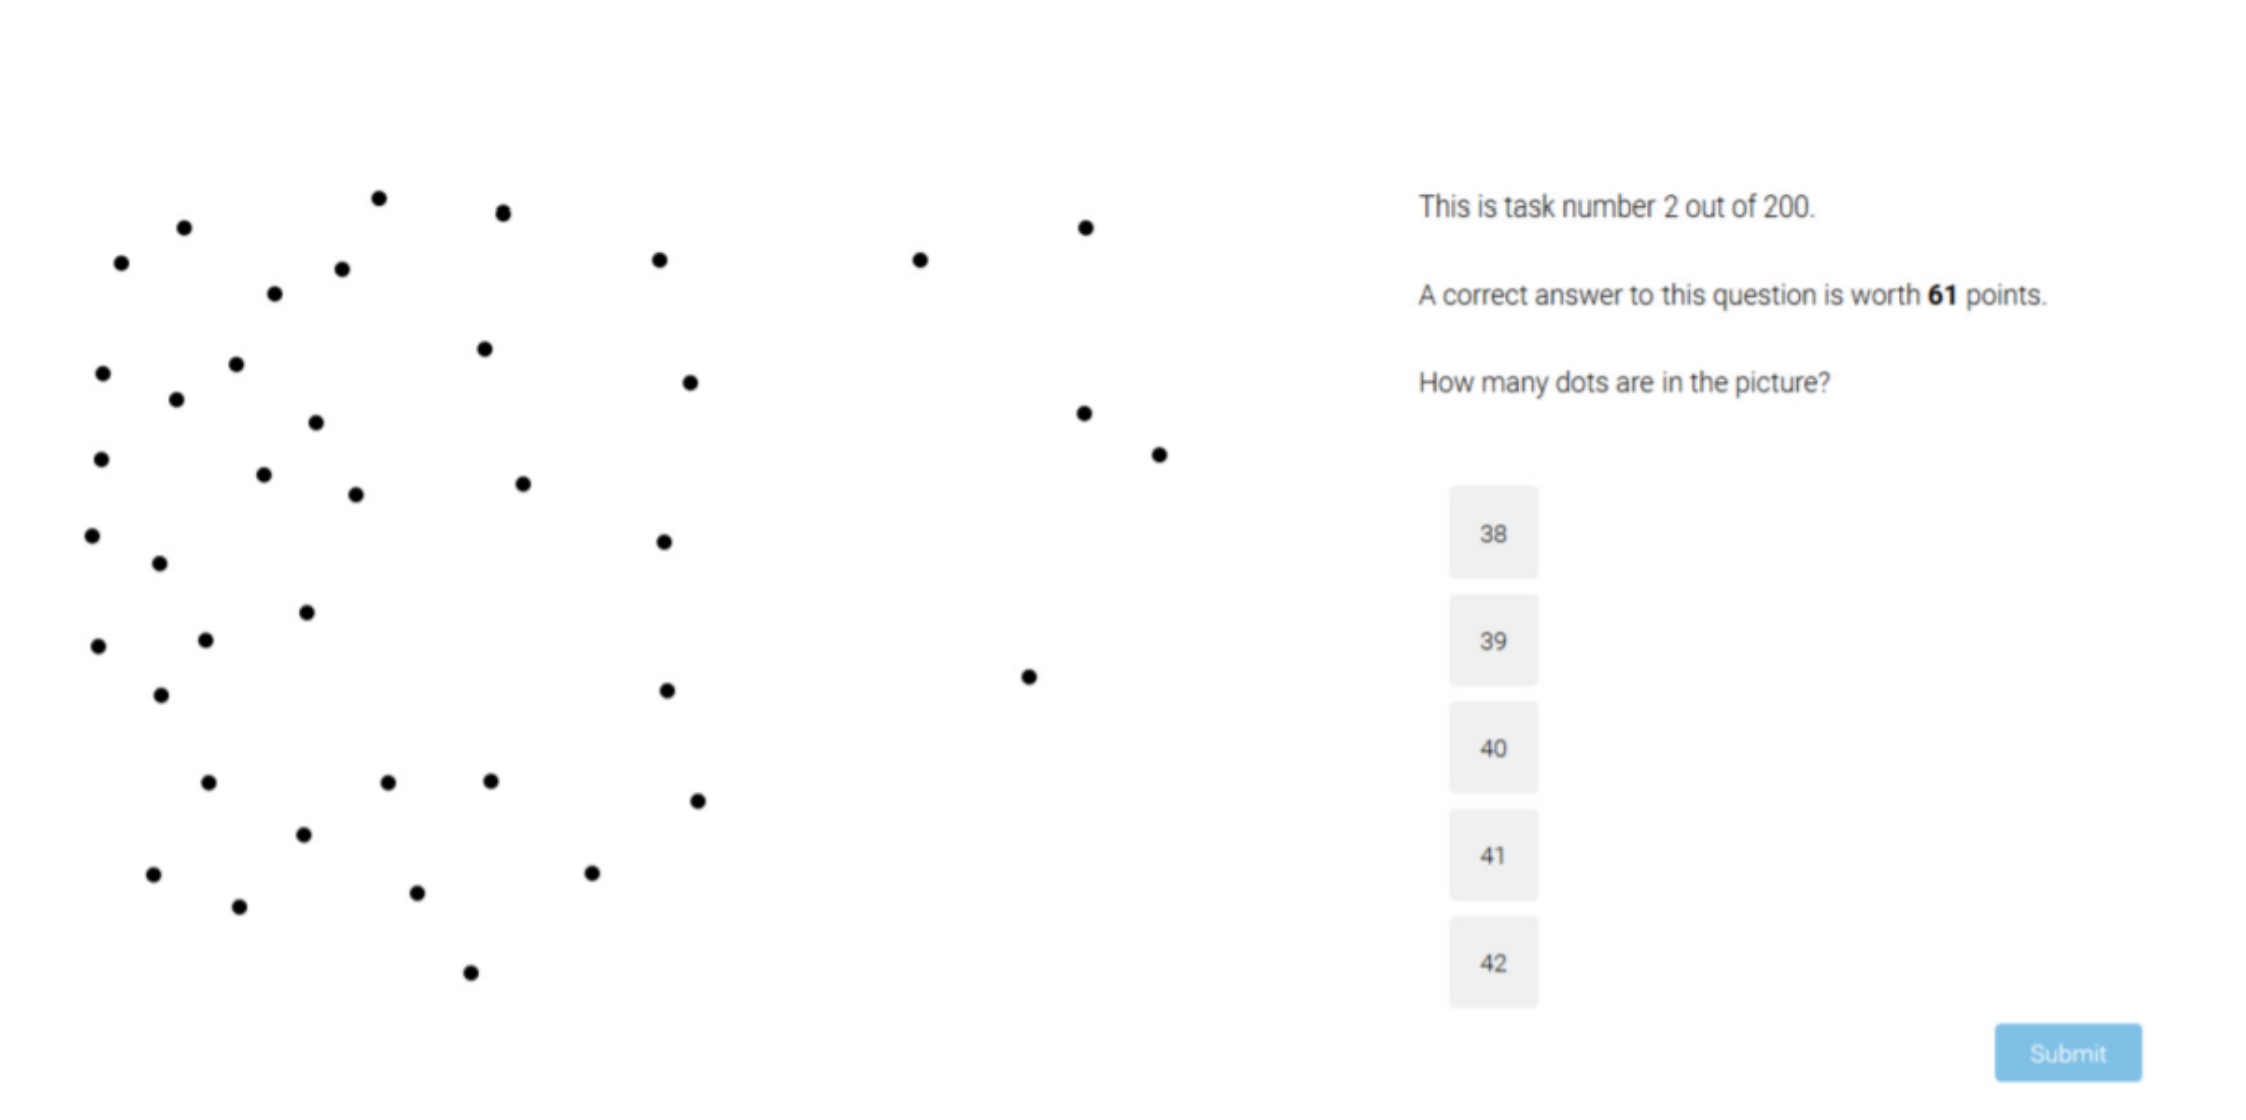
\includegraphics[scale=0.4]{IMAGEN DIST DE PUNTOS.png}
        \caption{Pantalla 2, Distribución de puntos}
    \end{figure}


Además, había un incentivo monetario dependiendo de la performance general de la experiencia. 41 sujetos los premios fueron de \$ 10 USD, y para los otros 40 sujetos, los premios fueron de \$ 20 USD. Además de una tarifa de participación de \$ 10.
Todas las sesiones se llevaron a cabo en el Laboratorio Experimental de Ciencias Sociales de Columbia (CELSS) en la Universidad de Columbia, utilizando la plataforma Qualtrics. Realizamos 8 sesiones con un total de 81 sujetos, quienes fueron reclutados a través del Sistema de Contratación Online para Experimentos Económicos (ORSEE) (Greiner, 2015).

\subsection{Experimento Propuesto}

La modificación del experimento original consta de incluir un segundo incentivo que mide la sustentabilidad de los proyectos. Para esto, la variable $r$ que mide el nivel de incentivo, será una función lineal $f(r)$ que considerará el nivel de incentivo económico $r_1$ y el nivel de incentivo sustentable $r_2$.
Para esto, se utiliza el mismo conteo de puntos, con la misma distribución y posibles respuestas correctas. La primera pantalla, muestra dos barras ubicadas en ambos extremos de la pantalla, que subirán dependiendo de a que nivel de incentivo equivalen. La barra del lado izquierdo color azul, representa el nivel de incentivo económico $r_1$, y la barra del lado dereho de color verde, representa el nivel de incentivo sustentable $r_2$, (como muestra la Fig. 4). 

\begin{figure}[h]
        \centering
        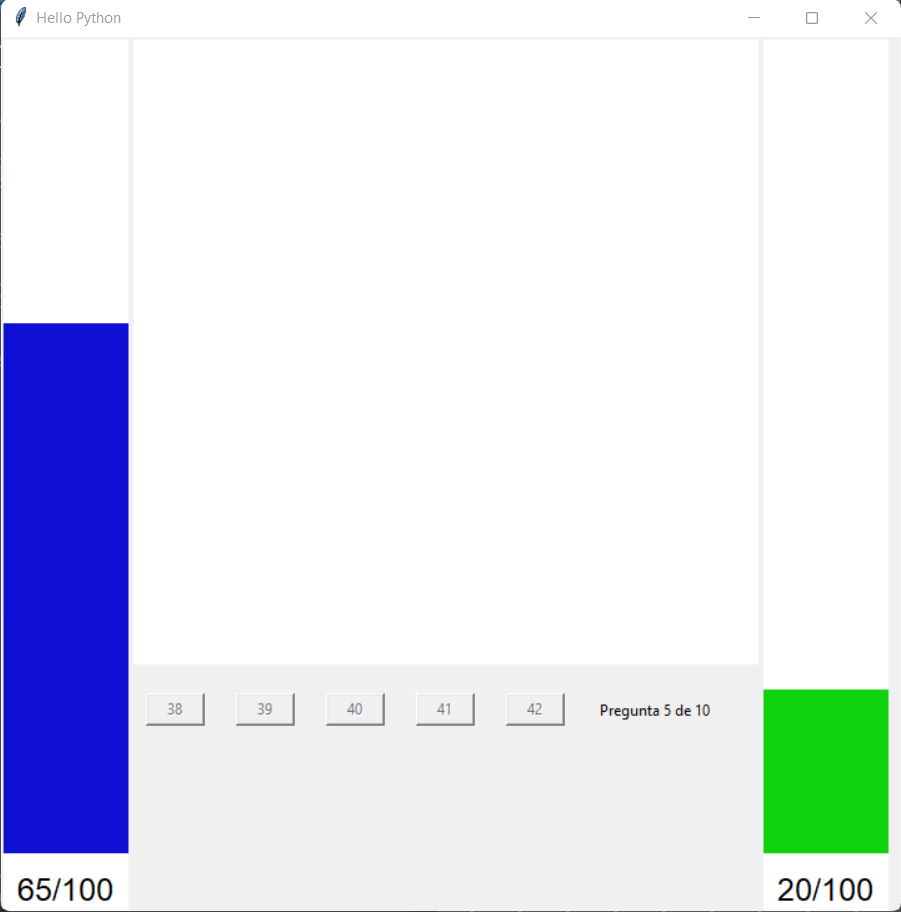
\includegraphics[scale=0.5]{pantalla 1 propuesto.png}
        \caption{Pantalla 1, Incentivos}
    \end{figure}

Los colores que se utilizan hacen referencia a los que comunmente se asocian a ambos retornos, dado que el color azul se asocia a un estado financiero sano y en general, por sobre algún valor crítico para las empresas y el color verde de la barra del nivel de sustentabilidad, se asocia a lo ecológico. Con esto, seguimos el hilo del experimento original buscando reducir al máximo las distracciones y el uso de la memoria en el momento de contar los puntos. 
Por lo mismo en la segunda pantalla, las barras permanecen visibles, mostrando siempre cuales son los niveles a los que se enfrenta el inversionista. Además, se muestra la imagen con la distribución de puntos entre 38 y 42 inclusive, y los sujetos podrán responder sin tener la limitante del tiempo al igual que en el experimento original (como muestra la Fig. 5).

\begin{figure}[h]
        \centering
        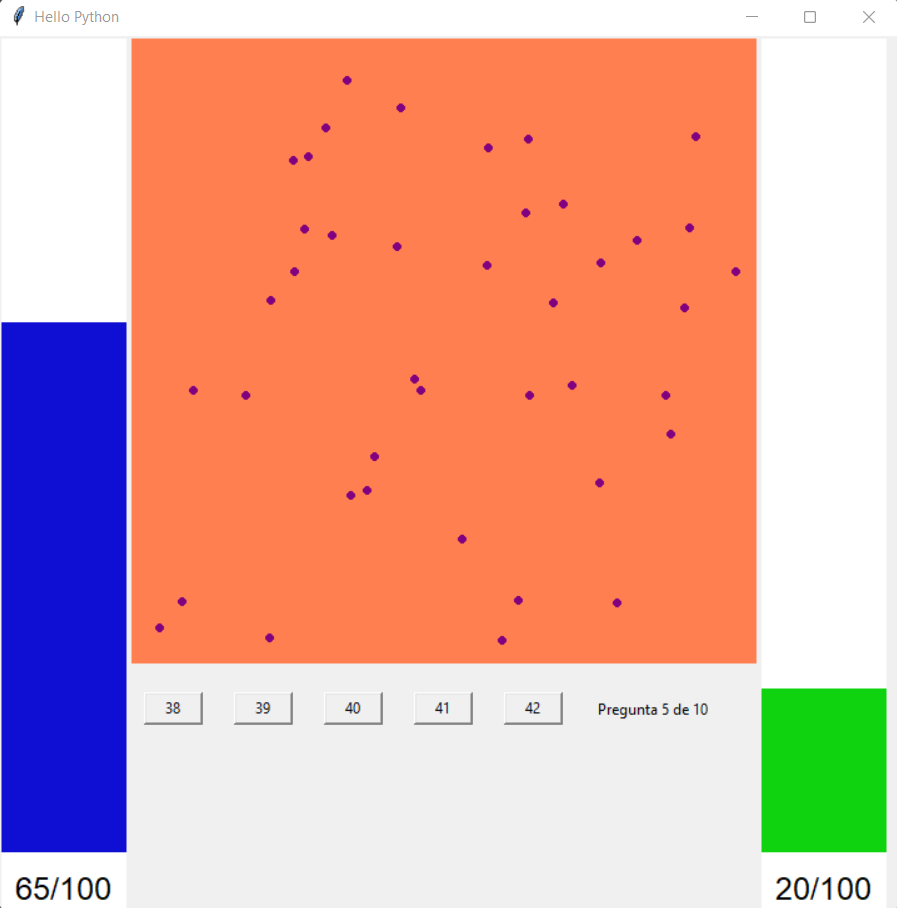
\includegraphics[scale=0.5]{pantalla 2 propuesto.png}
        \caption{Pantalla 2, Distribución de puntos}
    \end{figure}

Para lograr esto, se construyó un programa en lenguaje python, que será explicado más adelante y que se presenta en el anexo.

Ambos niveles de incentivo toman valores entre 1 y 100 inclusive, por lo que la suma de ambos puede dar un valor mayor a 100. Si los consideramos de la misma forma que en el experimento original, esto no tendría sentido ya que el porcentaje de probabilidad máxima de ocurrencia es 100\%. Además, tanto para la suma como para la resta, no se pueden repetir los niveles que aparecen en pantalla, y deben aparecer los 100 casos posibles. Para solucionar este problema y tener muchas combinaciones posibles entre los dos niveles, es que el ambos niveles de incentivo a nivel de programación pueden tener valores muchisimo mayores, pero que representaran un número de 1 a 100. En otras palabras, el programa busca 100 posibles combinaciones de incentivos iterando entre los números que tiene disponibles. Veamos un ejemplo: imaginemos que los un nivel de incentivo económico de 80 y un nivel de incentivo sustentable de 70. La suma de ambos, 150, representa el nivel de incentivo general 85 para ese individuo, dado que tiene 15 combinaciones entre incentivos más altas que 150 y 84 combinaciones de menor valor.

Con esto, aseguramos la aleatoriedad del experimento, así como la aparición de los 100 niveles de incentivos.

\subsubsection{Código Experimento Propuesto}

La versión de Python que se utilizó es la 3.9.7 de 64 bit. En primer lugar, es necesario descargar e instalar las librerías \textbf{\textit{tkinter, PIL, timeit}}. La primera funciona para la creación y el desarrollo de aplicaciones de escritorio, la cuál facilita el posicionamiento y desarrollo de una interfaz gráfica de escritorio con Python y es la que utilizamos para visualizar el juego. La librería \textit{Pillow} nos ayuda a trabajar con imagenes en distintos formatos. Por último, la librería \textit{timeit} mide distintos ciclos o tiempos de ejecución para pequeños fragmentos del código.

Además, se utilizán las librerías \textbf{\textit{random, threading, datetime, os, csv, time}}, las cuales son más estándar y vienen incluidos en el paquete inicial de la versión de python utilizada.

En la primera parte del código, se definen las funciones generadoras base \textit{generateCoords, generateIncentive, generateImage, generateSplash, generateEnding, generateProgressbar} (como muestran las Fig. 6 y 7).



\begin{itemize}
    \item \textbf{generateCoords:} Genera la distribución de los puntos y las coordenadas aleatoreas con las que aparecerán en la pantalla 1.
    \item \textbf{generateIncentive:} Genera la pantalla base donde irán los incentivos, no así las barras ni los niveles.
    \item \textbf{generateImage:} Genera la imagen donde irán los puntos y su distribución, la cuál ya fué obtenida por la función generateCoords.
    \item \textbf{generateSplash:} Genera el displey con las instrucciones del juego.
    \item \textbf{generateEnding:} Genera las variables que irán en el layout final del juego, entregando un resumen con los resultados más reelevante, como las respuestas corresctas, los puntos obtenidos y el tiempo que demoró en responder.
    \item \textbf{generateProgressbar:} Genera la imagen con los porcentajes y niveles de incentivo que muestra cada barra.
\end{itemize}

\begin{figure}[h]
        \centering
        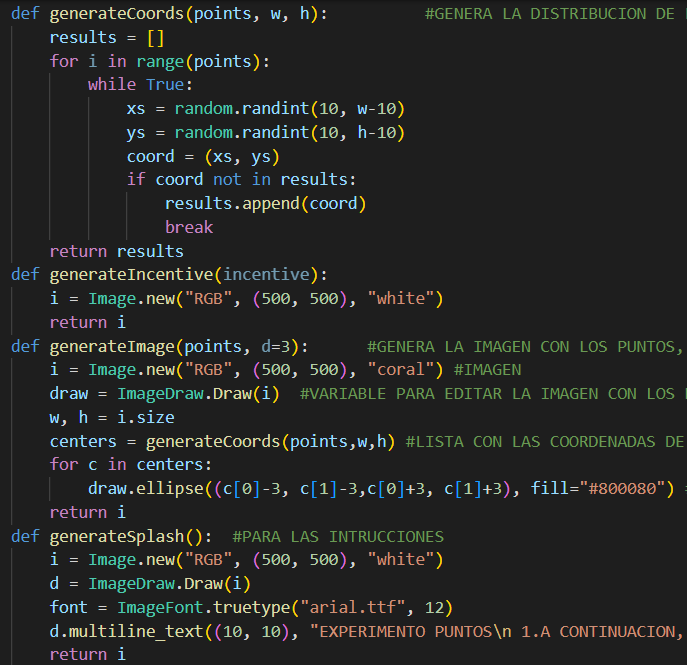
\includegraphics[scale=0.6]{gen 1.png}
        \caption{Funciones Generadoras parte 1}
    \end{figure}
    
\begin{figure}[h]
        \centering
        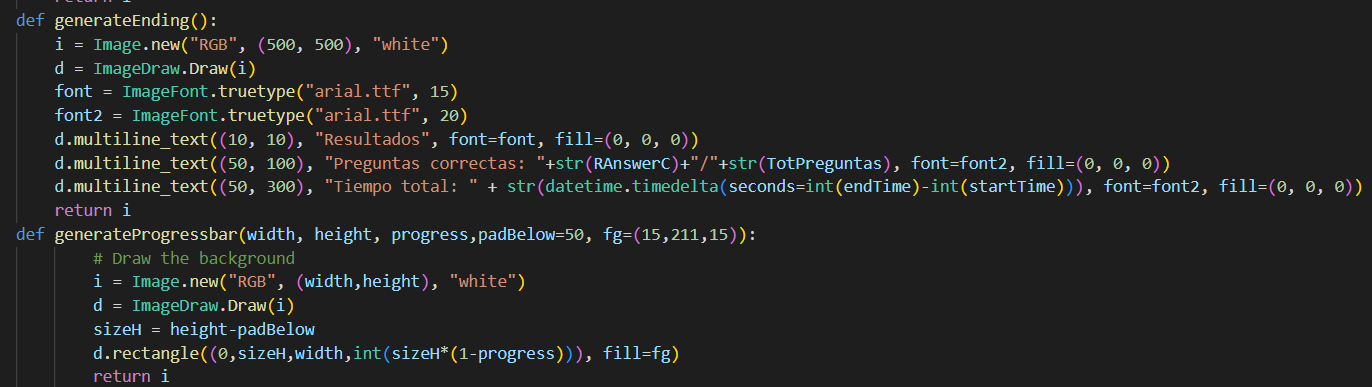
\includegraphics[scale=0.5]{gen 2.png}
        \caption{Funciones Generadoras parte 2}
    \end{figure}

La función \textbf{\textit{nextIm}} (Fig. 8) que inicia una vez que comienza el juego, al apretar el botón ``comenzar", suma el incentivo de la pregunta cuando es correcta, así como aumenta en una unidad el contador de preguntas, hasta que iguala la cantidad de preguntas totales de la experiencia.

\begin{figure}
 \centering
  \subfloat[Función nextIm parte 1]{
   \label{f:nextIm 1}
    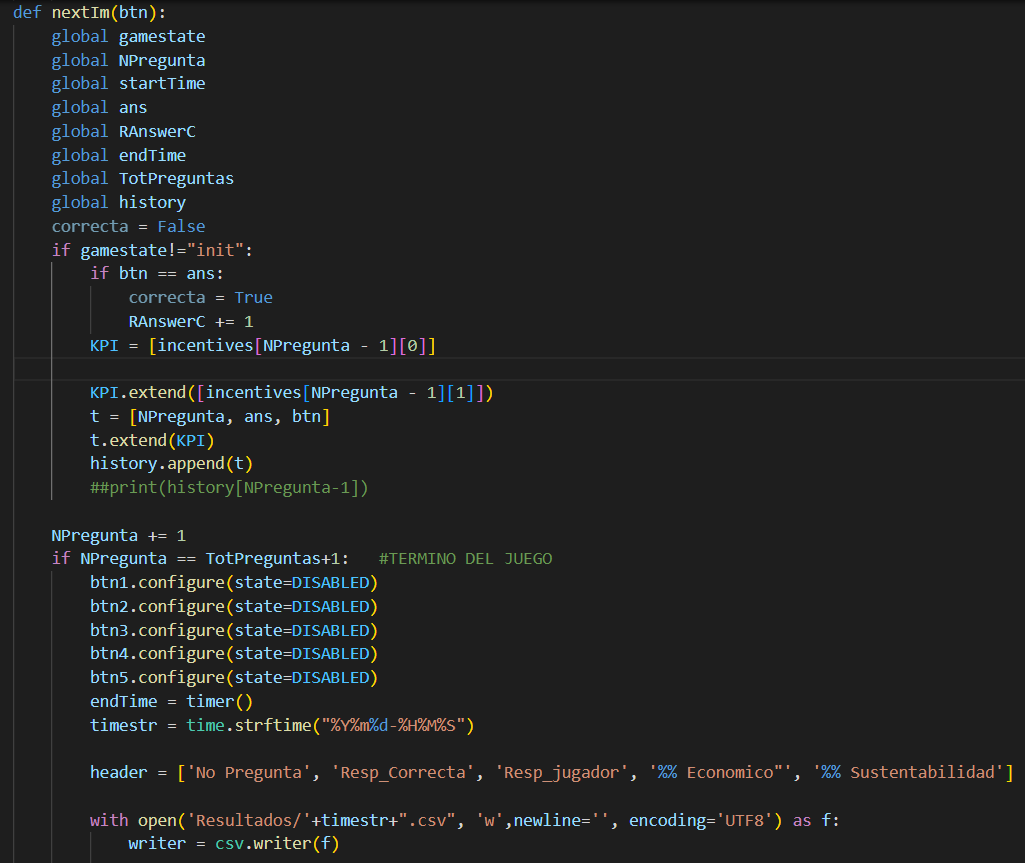
\includegraphics[width=0.5\textwidth]{nextIm 1.png}}
  \subfloat[Función nextIm parte 2]{
   \label{f:nextIm 2}
    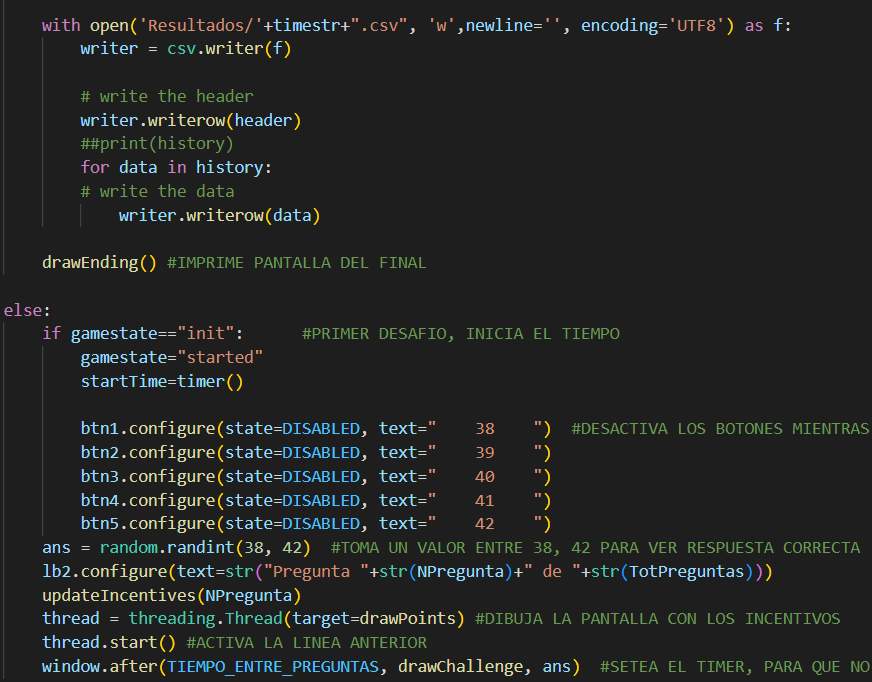
\includegraphics[width=0.5\textwidth]{nextIm 2.png}}
 \caption{Función nextIm}
\end{figure}


Luego, tenemos una serie de funciones \textbf{\textit{draw}} (como muestran las Fig. 9 y 10) con las cuales ``dibujamos" sobre las imagenes que generamos en pricipio los niveles de incentivos, además de activar los botones con las 5 posibles respuestas que tiene cada caso, que como ya vimos, pueden ser entre 38 y 42 inclusive. Estas funciones son \textbf{\textit{drawPoints, drawPercent, drawChallenge, drawEnding}}.

\begin{figure}
 \centering
  \subfloat[drawPoints]{
   \label{f:fig 6}
    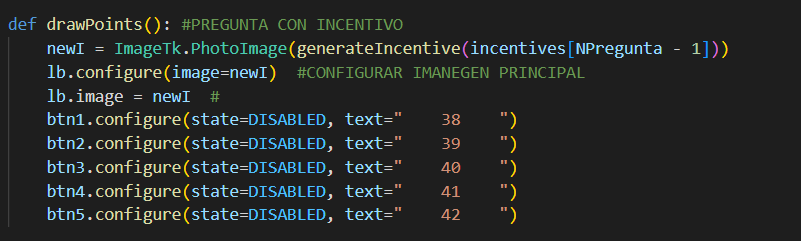
\includegraphics[width=0.5\textwidth]{fig 6.png}}
  \subfloat[drawPercent]{
   \label{f:fig 7}
    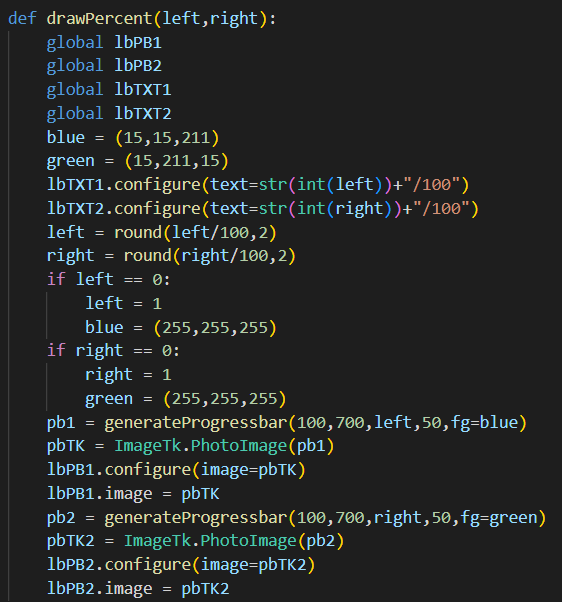
\includegraphics[width=0.5\textwidth]{fig 7.png}}
 \caption{Funciones draw parte 1}
\end{figure}



\begin{itemize}
    \item \textbf{drawPoints:} Dibuja los incentivos de cada caso, en particular los números que aparecen en la parte inferior de cada barra.
    \item \textbf{drawPercent:} Dibuja los porcentajes y las barras que están en los costados y representan los niveles de incentivos. 
    \item \textbf{drawChallenge:} Dibuja los puntos que ya fuerón distribuidos en las funciones generadoras.
    \item \textbf{drawEnding:} Dibuja el layout final con el cuadro resumen de la experiencia completa del individuo.
\end{itemize}

\begin{figure}
 \centering
  \subfloat[drawChallenge]{
   \label{f:fig 8}
    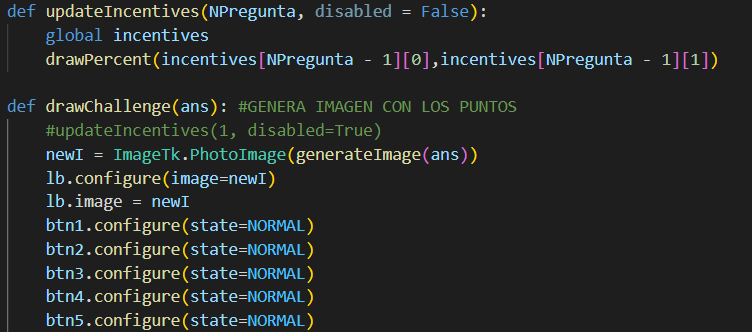
\includegraphics[width=0.5\textwidth]{fig 8.png}}
  \subfloat[drawEnding]{
   \label{f:fig 9}
    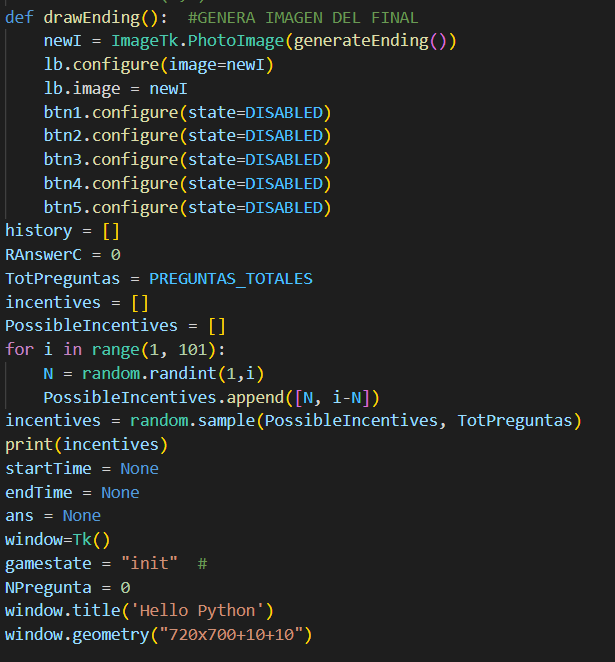
\includegraphics[width=0.5\textwidth]{fig 9.png}}
 \caption{Funciones draw parte 2}
\end{figure}


La figura 11, muestra las variables que generan las barras con los incentivos, junto con el texto que va debajo de cada barra mostrando de forma cuantitativa lo que representan, junto con la forma en que el código genera y presenta los botones con las opciones que tiene el individio para escoger según los números que cuenta.

\begin{figure}
 \centering
  \subfloat[Barras]{
   \label{f:fig 8}
    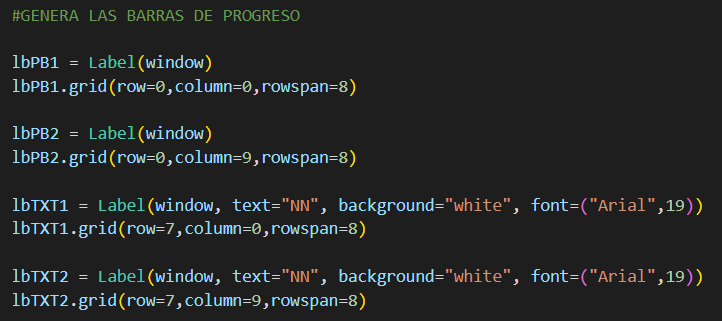
\includegraphics[width=0.5\textwidth]{barras.png}}
  \subfloat[Botones]{
   \label{f:fig 9}
    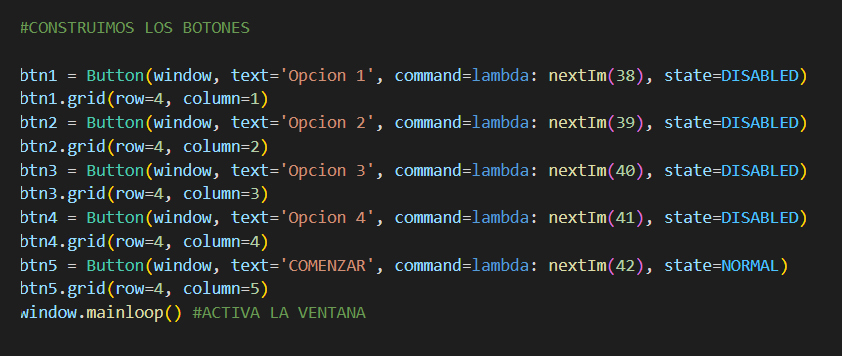
\includegraphics[width=0.5\textwidth]{botones.png}}
 \caption{Generador de barras y botones del layout}
\end{figure}

\subsection{Simulación del Experimento Propuesto}

Por distintas razones de tiempo y recursos disponibles, se tomó la decisión de utilizar los datos recolectados por Dewan y Neligh en su experimento, pero agregando la variable de sustentabilidad de forma símulada, dejando el resto de las variables "constante". 

Por ejemplo, considere un inversionista que en el experimento original se enfrentó a un nivel de incentivo $r = 60$ en el intento 4, la cantidad de puntos que mostró la pantalla era $n=39$ y respondió correctamente.
Con la modificación, el mismo inversionista estará enfrentado a una pantalla que muestra el mismo nivel de incentivo económico $r_1=60$, un nivel de incentivo $r_2=30$, la misma cantidad de puntos (39) y asumismo que respondió de forma correcta. Con esto, dependiendo de la funcioón lineal que usemos, $r$ toma otros valores. 
En este experimento solo se utilizarán dos funciones lineales. La primera será la suma de ambos niveles, por lo que si utilizamos el ejemplo anterior quedará: 

\begin{equation}
    f(r) = r_1 + r_2
\end{equation}
\begin{center}
    f(r) = 60 + 30 = 90
\end{center}


Analogamente, la segunda función será la resta, y utilizando el ejemplo anterior queda:

\begin{equation}
    f(r) = r_1 - r_2
\end{equation}
\begin{center}
    f(r) = 60 - 30 = 30
\end{center}

Esto es muy interesante de analizar, ya que si originalmente al tener un $r = 30$ el sujeto contestaba de forma incorrecta, en el caso de utilizar la segunda función de r, para la simulación estará contestada de forma correcta (recordemos que para $r = 60$ en el problema original el TD contestaba correctamente según el ejemplo). La hipótesis que postulamos, es que un nivel de incentivo sustentable más alto, podría conllevar un menor nivel de incentivo económico, y por lo tanto el tomador de decisión deberá escoger cuál de estos dos atributos es el más importante.

\subsection{Base de datos}

La base de datos para poder desarrollar la simulación, se construyó utilizando algunos valores de la tabla original. Estos valores son los siguientes:

\begin{itemize}
    \item \textbf{trueDots:} son todas las respuestas correctas en cada oportunidad que los invidividuos debieron contar puntos. Como ya fué explicado, son 100 experiencias por cada participante, y son 80 individuos.
    \item \textbf{incDots:} es el nivel de incentivo que apareció cada ves que un individuo se vió enfrentado al conteo de puntos
    \item \textbf{choseDots:} es la alternativa que escogió el TD en cada oportunidad
\end{itemize}

A partir de estos valores, se simuló de forma aleatorea la variable \textbf{\textit{incDots\_S}} la cuál puede tener valores de 1 a 100 inclusive, y su construcción está explicada en la sub sección 4.4.1 y corresponde al $r_2$ (nivel de incentivo sustentable), y la variable \textbf{\textit{incDots}} ahora tomará el nombre de \textbf{\textit{incDots\_E}} que corresponde a $r_1$ (nivel de incentivo económico).

La variable \textbf{\textit{incDots\_suma}} corresponderá a la suma de $r_1 + r_2$ (suma de los incentivos sumados) o \textbf{\textit{incDots\_resta}} a la resta de ambos incentivos dependiendo del análisis que se esté realizando.

También, la base de datos contiene una columna con los costos estímados para cada uno de los individuos (como muestra la Fig. 12). Esta variable se obtiene luedo de estimar los betas necesarios para la función de costos cuadráticas, aplicando la regresión que mejor se ajusta como vimos en el capítulo 4, y como se explica en la sección 5.6. 



Con esto, la base de datos queda constituida de la siguiente manera:

\begin{itemize}
    \item \textbf{Columna 1:} incDots\_E, dependiendo de cuál caso se evaluó a cada participante.
    \item \textbf{Columna 2:} incDots\_S, dependiendo de cuál caso se evaluó a cada participante.
    \item \textbf{Columna 3:} incDots\_suma o incDots\_resta de ambos casos.
    \item \textbf{Columna 4:} costE\_suma o costE\_resta, costos estimados para ambos casos.
    \item \textbf{Columna 5:} trueDots\_E, la respuesta correcta cuando el caso evaluado corresponde al que evalua el incentivo económico. 
    \item \textbf{Columna 6:} choseDots\_E, la respuesta que eligió el individuo cuando el caso evaluado corresponde al que evalua el incentivo económico.
    \item \textbf{Columna 5:} trueDots\_S, la respuesta correcta cuando el caso evaluado corresponde al que evalua el incentivo sustentable. 
    \item \textbf{Columna 6:} choseDots\_S, la respuesta que eligió el individuo cuando el caso evaluado corresponde al que evalua el incentivo sustentable.
\end{itemize}

insertar imagen de la base de datos final para la suma y la resta.

\subsubsection{Contrucción variable incDots\_S}

Esta variable debe cumplir una serie de restricciones para que tenga sentido tanto la simulación como el experimento propuesto. Recordemos que las variables de los incentivos pueden tener valores entre 1 y 100 inclusive, deben aparecer todos los valores, y deben aparecer de forma aleatorea. Para poder cumplir lo anterior, se vuelte imposible que la suma de ambos incentivos den los números del 1 al 100, por lo tanto, se tomó la decisión de ampliar el margen de la segunda variable $r_2$, generando 100 números aleatoreos, que ordenados de menor a mayor, corresponderan a uno de los 100 porcentajes que deben estar presentes para cada individuo. Para explicarlo de mejor manera, se muestra el siguiente ejemplo. Imagine los 3 

La variable \textbf{\textit{incDots\_S}} se gener

\subsection{Estimación de los betas}

Para poder realizar este analisis y ser concluyentes con la simulación que se plantea, se harán diferentes estimaciones aplicando modelos de regresión lineal y multiples. 

Se utilizaron los datos obtenidos por los autores Dewan y Neligh (2019), que se encuentran en el anexo... Es una base de datos muy completa, con datos específicos de tiempos, resultados, entre otros. En el desarrollo de esta simulación, solamente utilizaremos los siguientes dato:

\begin{itemize}
    \item \textbf{trueDots:} son todas las respuestas correctas en cada oportunidad que el TD debió contar puntos. Como ya fué explicado, son 100 experiencias por cada participante, y son 81 individuos.
    \item \textbf{incDots\_E:} es el nivel de incentivo económico que apareció cada ves que un individuo se vió enfrentado al conteo de puntos
    \item \textbf{choseDots:} es la alternativa que escogió el TD en cada oportunidad
    \item \textbf{incDots\_S:} es el nivel de incentivo sustentable que se simuló para cada experiencia realizada por el participante.
\end{itemize}

Con respecto a este ultimo valor, se simulan datos que tienen ciertas restricciones para poder mantener la válidez del experimento. En primer lugar, la suma del incDots\_E, que llamaremos $r_1$, con el incDots\_S, que llamaremos $r_2$ no puede ser superior a 100. Esto, porque como se señaló anteriormente, los niveles de incentivos son probabilidades, y por tanto, una probabilidad superior a 1 (o 100 por ciento posible) sería irrelevante, o nos daría la misma información que la máxima probabilidad de ocurrencia.. Además, deben aparecer todas las probabilidades, es decir, desde el 1 hasta el 100 inclusive. 
De esto ultimo, se desprende la segunda restricción con respecto a la segunda variable de retorno, $r_2$, donde debe ser tal, que al sumarlas, aparezcan todos los casos.
De forma analoga, cuando se restan los incentivos, tampoco puede ser menor a 0.
Más adelante, se explica a través de una modelación matemática lo anteriormente explicado.
Para avanzar con el experimento, y apegandose al original, se tomaron en consideración dos respuestas o \textit{choseDots}, una del nivel inferior, es decir, cualquier nivel de incentivo sumado igual o inferior a 50, y otra del nivel superior, es decir, cualquier nivel de incentivo sumado superior a 50.
Con esto obtenemos las variables \textbf{incDots\_suma} o \textbf{incDots\_resta} dependiendo del caso.
La siguiente variable que vamos a obtener, es la variable \textbf{perf}, que será la performance de cada participante. Esta será igual a la suma de las respuestas correctas de cada inviduo entre las dos que serán seleccionadas al azar para cada uno de ellos.
Por ejemplo, imaginemos al inviduo numero 30, cuyas respuestas evaluadas son para un nivel de incentivo sumado igual a 15 (nivel inferior, caso 1) e igual a 75 (nivel superior, caso 2). En el caso 1, el \textbf{incDots\_E} es igual a 10, y el \textbf{incDots\_S} es igual a 5. Por otro lado, en el caso 2, el \textbf{incDots\_E} es igual a 40, y el \textbf{incDots\_S} es igual a 35.  Además, sabemos que el TD respondió correctamente el caso 2, e incorrecto el caso 1, por tanto su performance (\textbf{perf}) es igual a 75. Todos estos datos, los podemos observar de mejor forma en la figura 4.


\begin{figure}[h]
    \centering
    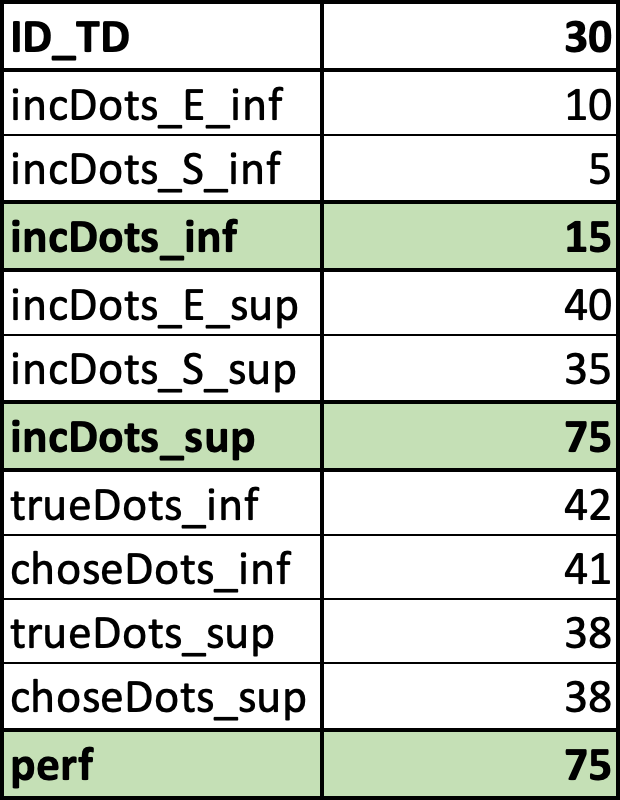
\includegraphics[scale=0.4]{TABLA DATOS EJEMPLO.png}
    \caption{Tabla de datos ejemplo}
\end{figure}



Se utilizarán distintas regresiones lineales para estimar los betas, donde $P_t$ es la performance del TD, y el $r_t$ es el nivel de incentivo sumado o restado./












\section{Conslusiones}




\vspace{3cm}


Nota (escala 1 a 7): 
\vspace{3cm}
Observaciones



\centering Firma Guía



    






\newpage











































%ejemplo Plantilla



\end{document}
https://www.overleaf.com/project/62b5d06662bca87393f4c7d7